%===================================== CHAP 3 =================================

\chapter{Research Method}\label{chap:4}

The Oates'\cite{oates2005researching} model of the research process was used as a guideline for selecting the research method in this project. The model and the specific methods chosen is displayed in Figure \ref{fig:research_process}. This process will be used as the outline for the structure of this chapter.

\begin{figure}[H]
    \centering
    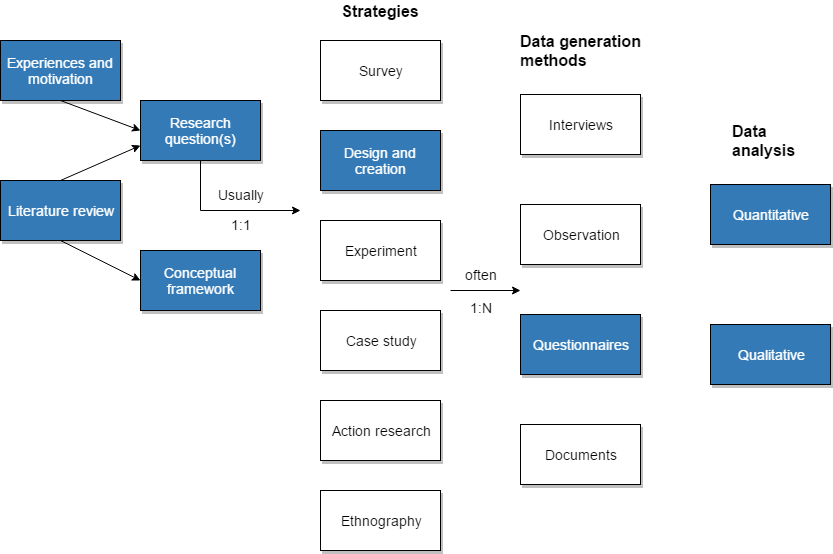
\includegraphics[width=0.9\textwidth]{fig/research_process.png}
    \caption{The outlined research process}
    \label{fig:research_process}
\end{figure}

As summarized in section \ref{RQ} the purpose of this project is to study the use of CBR in an information system and its effects on students motivations for doing an exchange or study abroad program. As according to Oates'\cite{oates2005researching} model the research questions were formed after identifying the purpose, motivation and related work through literature review. The research questions, see section \ref{RQ}, can be answered by evaluating an artefact created through the design and creation strategy. The final evaluation will be done using both qualitative and quantitative data analysis on data gathered from data generation methods such as an offline experiment of recommender system and questionnaires.

\section{Research Strategy: Design and Creation}

This research will use the design and creation strategy to develop a computer based artefact named Utsida. Utsida will be used as a tool to answer the research questions detailed in section \ref{RQ}.   

Utsida will consist of two systems, a case-based recommender system (CBRS) back-end and a web application which will serve as the platform users meet. The system as a whole will be created as a tool to generate the data needed to answer both RQ1 and RQ2. It will incorporate the AI methodology CBR to create a new way of recommending relevant universities and courses for a student applying for an exchange- or study abroad program. The web application will also serve as the page for choosing, approving and managing course applications that could influence the students motivation.

To be able to answer RQ2, the system needs to be well functioning and easy to use. Therefore it is beneficial to use the design and creation strategy to assist with the development of the system. The design and creation will be done in an iterative process according to the five steps from Vaishnavi and Kuechler (2004)\cite{vaishnavi2004design}: Awareness, Suggestion, Development, Evaluation and Conclusion.

\subsection{Awareness and Suggestion}
Awareness is the part of finding and defining the problem domain, done in the preliminary research in chapter \ref{chap:2} and through the research questions, section \ref{RQ}. When the problem has been identified, a suggestion for the system will be made. This suggestion includes the first design details for the system, and then the development process will begin. 


\subsection{Development}

To answer the research questions, data generated by real users is necessary. It was therefore essential that the web application part of Utsida, especially the front-end, is easy and intuitive to use. To ensure this, the development of Utsida will be done in an iterative manner. This includes communication with potential users throughout the development, and also usability testing. B. W. Boehm (1988)\cite{boehm1988spiral}, presented the \emph{Spiral Model}, which is now a common model for iterative development where each cycle includes analyzing risks and requirements, development and testing of a prototype, planning the next iteration, and determining the objective of the next iteration. This model fits well this research, so an adaption of this model was chosen as the designated development methodology. Figure \ref{fig:development_process} displays the adapted version of the spiral model, where the main differences are less risk assessment and verification and validation of each prototype. The reasoning for this is that it is necessary to quickly try out ideas and functionality and get them tested to see if they are feasible. Furthermore, as this is a relatively short-term project, there will be limited time available for analysis and validation between each cycle.

\begin{figure}[h]
    \centering
    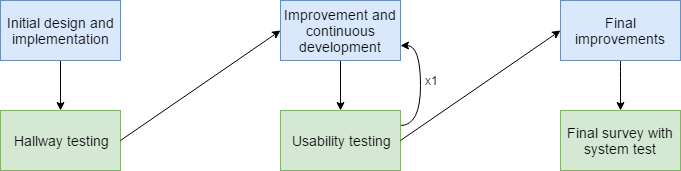
\includegraphics[width=1\textwidth]{fig/development_process.png}
    \caption{The development process of Utsida, an adaption of the spiral model\cite{oehm1988spiral}}
    \label{fig:development_process}
\end{figure}

\subsection{Evaluation and Conclusion}
Evaluation will be done continuously after each development cycle and the whole process redone if found needed. Part of the iterative evaluation will be done by testing the system on students through usability tests and hallway testing. The final evaluations will be achieved through an online test with an accompanying questionnaire, as well as performing an offline experiment detailed further in section \ref{sec:questionnaire_1}, \ref{sec:questionnaire_2} and \ref{sec:observation_test}.

\subsubsection{Usability Testing}

Iterative sessions of usability testing will performed on the web application to evaluate and ensure sufficient usability. The test participants will be selected carefully and will consist mainly of students who have a decent understanding of the current approach for applying for an exchange program. Both technical competent- and less technical competent students will be tested.

These tests will help finding flaws in both general functionality and design, so that the system is as reliable as possible before conducting the remote online test. Data will be gathered by interviewing the testers, observing their use of the system, and have them fill out a System Usability Scale (SUS)-schema\cite{brooke1996sus}. After each test, this data will be analyzed using the SUS score\cite{brooke1996sus} with a range from 0 to 100.

\section{Data Generation Methods}
Because there is no client, or persons with high stakes in this project, interviews are not viewed upon as a feasibly method to generate data. There is no existing documents which may be reviewed to gather the required data. Questionnaires and experiments are common methods to generate data about a software system\cite{oates2005researching}, and suits the desires of obtaining generalized opinions about a software system's effect and functionality, and is therefore chosen as the designated data generation methods. 

\subsection{Questionnaires}

Questionnaires will be used as the main method for generating data for the research questions. Two questionnaires will be used to answer the research questions in this project. The first one will be conducted during the development of the system with the goal of learning what students think are the most important motivational factors for choosing an exchange location, see section \ref{sec:questionnaire_1} for further details. The second questionnaire will be conducted after the system prototype is complete as a final evaluation, and will be accompanied with a remote user test. All the design details of the second questionnaire can be found in section \ref{sec:questionnaire_2}.

Both questionnaires will be self-administrated, which promotes the opportunity to collect data from a larger number of students at once. This method also suits the limitations of this project well with low cost and lower time usage for conducting and planning the test compared to administrated tests. The recipients of the questionnaire will be students who have some experience with exchange studies. To acquire a larger target group who fits this criteria NTNU's Office of International Relations will be contacted for possible access to email lists and Facebook sites.

The majority of the questions in the questionnaires will be closed questions, and the question forms which will be used for these are the likert scale\cite{allen2007likert}, semantic differential scale\cite{osgood1952nature} and questions with \enquote{Yes}, \enquote{No}, or \enquote{Don't know} options. According to Dawes J. G. (2012)\cite{dawes2012data}, the results from using a 5-point- and 7-point scale are very similar. Questionnaire 1 will use a scale from 1-7 while questionnaire 2 will use a 1-5 scale. A 1-7 scale was chosen to better fit the model in MyCBR workbench were the weights are represented from 1-10. While the 1-5 scale will represent the level of agreement in the question statement, and fits well with the possible answers, see figure \ref{fig:q2_question_form}. In addition, there will be asked a few open questions where the students can articulate their opinions freely if they like.

\subsubsection{Validity and Reliability}
Content validity is concerned with whether the questions in the questionnaire represents a good sample of the domain to be investigated\cite{oates2005researching}. The means that the selected questions should cover all the different evaluations needed to answer the research questions properly. Feedback from potential participants and experts where used to evaluate the validity. For RQ1 the main aspect is the "suitability" and whether the system recommends viable universities and courses. The expectation the user has in the usage of the system is also a factor that evaluates the suitability. RQ2 concern the effect on motivation of the students, and here the most important evaluations are use of the system, motivation effect and recommendation to others.

Construct validity means that the questionnaire is evaluating what it was intended to evaluated and not other aspects\cite{oates2005researching}. Questionnaire 1 and 2 were designed to ensure the construct validity by using clear and simple questions that targeted the specific aspects of the research questions. An iterative process was followed in the design of the questionnaire to remove or edit possible irrelevant and poorly formulated questions. 

The measurement of reliability is that the questionnaire yields the same result when given to the participants repeatedly. This is difficult to asses as the questionnaire will only be given once and the participants does not evaluate the system over time. Evaluating the system over time with part of participants would also distort the data by giving them more time to be familiar with the system. However, one way to measure the reliability of the internal consistency is using Cronbach's alpha.\cite{bland1997statistics}

\subsubsection{Bias}

By using questionnaires as the main method to collect data, several risks of bias is introduced. When designing the questions, measures to minimize implicit bias will be done. The majority of the questions will therefore strive to be neutral statements which the participants can state their degree of agreement as given by the Likert scale\cite{allen2007likert}. Furthermore, the target population for the questionnaires will be students who are interested in exchange in some way, which might influence responses to be more positive. 

Central tendency bias is a risk when the questions have extreme response categories, especially in the likert scale and semantic differential scale. A lower point scale will be used in questionnaire 2 to reduce the central tendency and both questionnaires will have clear questions that reduce the confusion of the participants and their likelihood of answering in the middle sections. 

Acquiescence bias is when the participant is likely to answer positively on a question.\cite{cronbach1946response} To reduce the acquiescence bias the questions should avoid being very positively based. However due the nature of the questions having less social desirability and not being sensitive a acquiescence bias is less likely to have a large impact. This is the same for social desirability biases.  

Considering the expected response rate will be a very small rate of the full population, non-response bias is unavoidable. There could be a general difference between the opinions of those who choose to answer the questionnaire and those who do not. Those who did not participate might think the research sounds uninteresting, and if they actually participated they might respond with more negative answers. Non-response bias will be taken into consideration when analyzing the final result data, and in the discussion.



\subsection{Questionnaire 1: Motivational Factors}\label{sec:questionnaire_1}

The goal of questionnaire 1 is to gain knowledge on important factors for students when they choose an exchange location and university. The results from this questionnaire will be the basis for the weighting of the attributes in the CBRS and choosing which attributes to include in the system. The target population is all Norwegian students that have either been on exchange or is considering going on exchange. This means they will have some background and considerations about their motivational factors. The total population size of questionnaire 1 is difficult to estimate since it also includes students that are considering going on exchange. However the goal of the sample size is 100 students to ensure some variability in the answers. A higher sample size is difficult to be obtained due to limitations in funds, time and access to publication sources for the questionnaire. 

%Skriv om statistic significance, confidence interval osv

The main question in questionnaire 1 is a closed question and it was formed according the semantic differential scale, see figure \ref{fig:semantic_scale}. The participant ranks each motivational factor according to the particular decisiveness of that factor. See appendix \ref{app:questionnaire1} for all the questions included in questionnaire 1. 

\begin{figure}[h!]
    \centering
    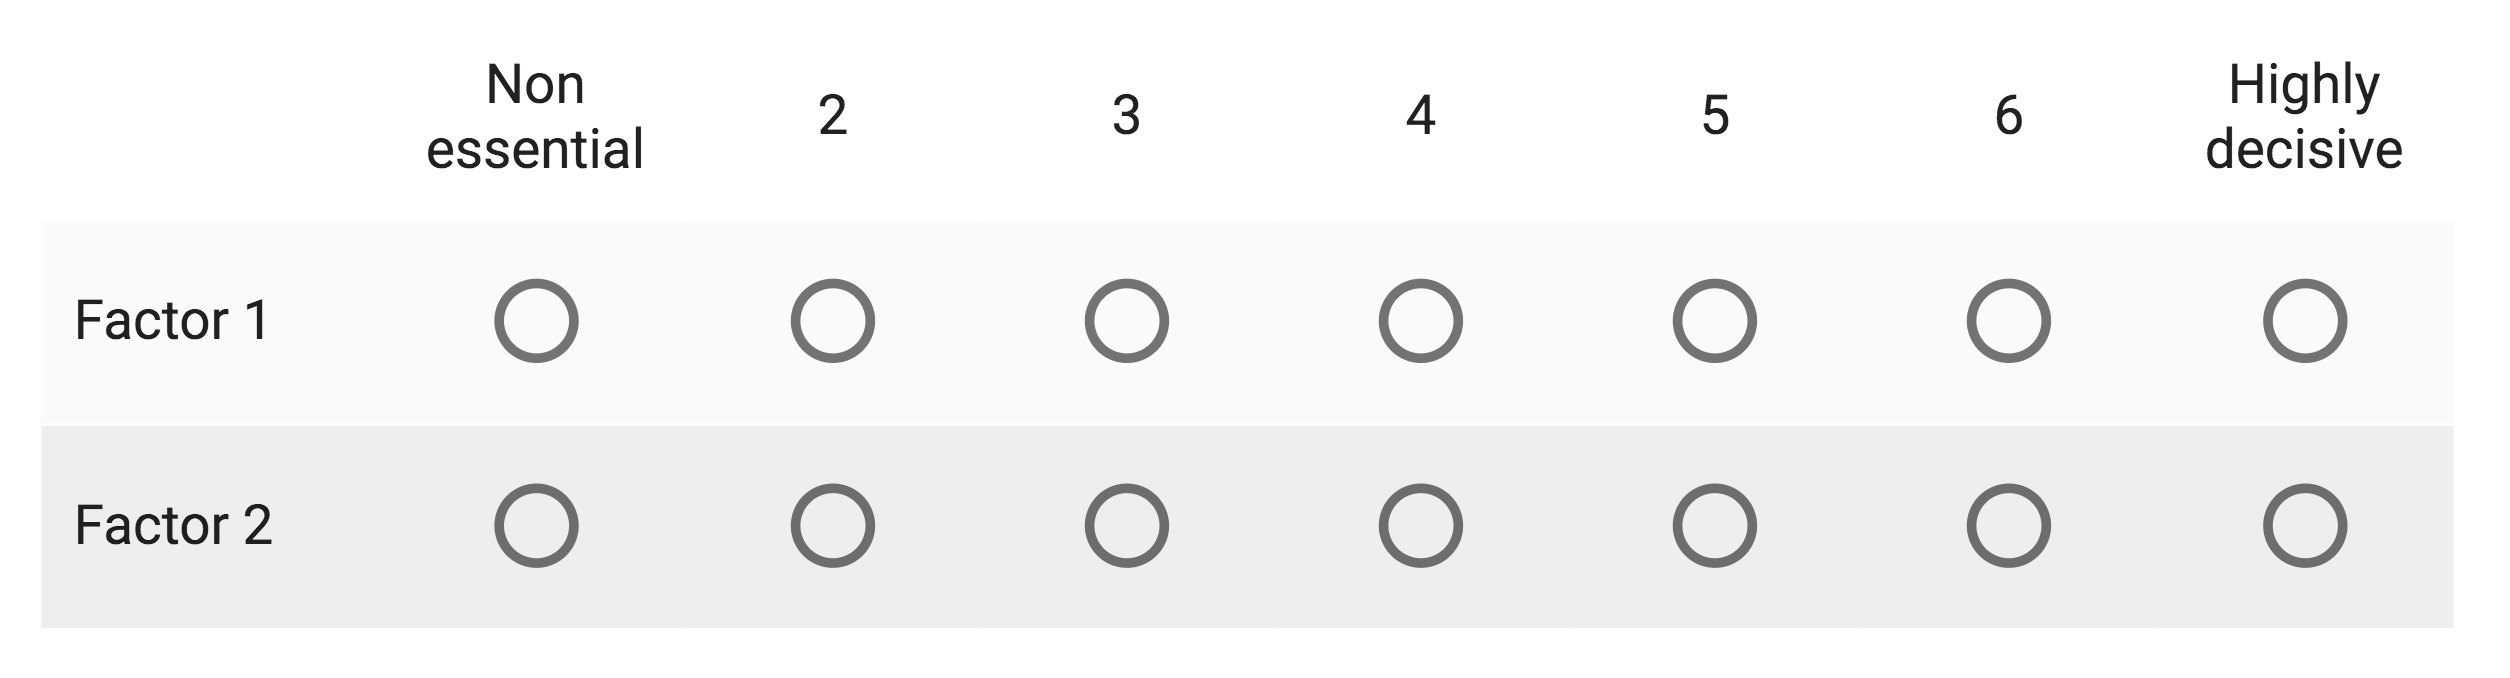
\includegraphics[width=1\textwidth]{fig/question1.png}
    \caption{Motivational factor weighting}
    \label{fig:semantic_scale}
\end{figure}

This questionnaire will also include an open ended question asking the students for feedback on possible other motivational factors that could be included in the system.

\subsubsection{Data analysis}
The numerical data from the questionnaire will be analyzed in a quantitative manner, by calculating the mean, standard deviation and coefficient of variation for each attribute. The coefficient of variation will be calculated to show the spread relative to the mean of the data and to rank each attribute against each other for the weighting purposes. Even though the data is original ordinal it will be analysed as interval data to fit with the weighting in the CBR model. 

The open ended text question will be analyzed in a qualitative manner by using theme analysis. First each question will be reduced to only include important sections related to the goal of the question and all unrelated parts will be removed. Then each answer will be analyzed by finding related themes of each question and mapping them in a table. The number of occurrences of a theme will then be counted and each theme ranked by importance. 

\subsection{Questionnaire 2: User Testing of Utsida}\label{sec:questionnaire_2}

The three goals of questionnaire 2 is to; 1. Evaluate and analyze how this system affects students motivation for applying for a study exchange- or study abroad program, 2. whether students who have already been on an exchange thinks this system would make their process easier, and 3. If the system delivered relevant recommendations to the user.

In order to keep the margin of error to a minimum it is important strive to get feedback from as many students as possible. Considering the limitations of budget, time and that the main questionnaire accompanied with a remote user test will take approximately 20 minutes, a goal of 60 answers is set. The questionnaire will be published through social media, and it will be attempted to cooperate with NTNU Office of International Relations, and have them publish it on their Facebook page which currently have about 3300 followers- all being in the target group of this research.

The questionnaire will consist of two main parts of questions, one for reviewing the motivation and use of the application and the other to evaluate the recommendation engine.

%Spørsmålsform, målgruppe, mål, hvordan det skal bli gjennomført, publiseringsmetoder, innsamling, data simplifisering?

\subsubsection{Part 1: Motivation and Use}
The questions in the first part of this questionnaire will be formed as a slight adaption of the Likert Scale\cite{likert1932technique}. This question form is designed as a five-point scale where each option represents a degree of agreement to a given statement. This way, the questions can be neutral statements, where the recipients of the questionnaire can select their the level of agreement they relate themselves the most with, leaving as little room for bias as possible. 

\begin{figure}[H]
    \centering
    
\includegraphics[width=1\textwidth]{fig/q2_question_form.PNG}
    \caption{The question form used in the first part of the questionnaire. Each question is lead by a statement regarding motivation.}
    \label{fig:q2_question_form}
\end{figure}

The questions in the first part of this questionnaire will ask about the motivational effect Utsida may have on their thoughts about applying for a study exchange- or study abroad program. Depending on weather the student has already been on a study exchange, or if they think about doing it, they will receive slightly different questions.

\subsubsection{Part 2: Evaluation of Recommendation}

The second part of the questionnaire will focus on the students evaluating the recommendations they receive from Utsida, as well as evaluating the results from two pre-defined queries to the CBRS. The question form will be designed to have simple \enquote{Yes}, \enquote{No}, \enquote{Don't know} answers to easier determine the amount of students that receive relevant recommendations. The pre-defined query recommendations will also include a question which asks the students to rate the recommendations (see Figure \ref{fig:q2_rate_search}). The pre-defined queries, see Appendix \ref{pre_defined_search_table}, are included to evaluate the recommendations for a specific search that does not rely on user input, and thus yields objective evaluation. 

\begin{figure}[H]
    \centering
    
\includegraphics[width=1\textwidth]{fig/rate_search.png}
    \caption{Question form on the suitability of a pre-defined search}
    \label{fig:q2_rate_search}
\end{figure}


\subsubsection{Data analysis}
This questionnaire will perform a data analysis similar to questionnaire 1 by using quantitative analysis on the closed questions and qualitative analysis on the open-ended question. The closed questions likert scale will be analyzed by the use of mode and frequencies. On the \enquote{Yes}, \enquote{No} or \enquote{Don't know} questions however, only percentages and number of answers for each option will be gathered. Cronbach's alpha will be used to asses the internal consistency of the likert scale questions on motivation. 

\subsection{Offline experiment of Recommender System}\label{sec:observation_test}
An offline experiment of recommender systems method introduced by Ricci et al.\cite{ricci2011introduction} will be used to test the technical part of the CBRS without user influence. This is a specific method to evaluate recommendation systems in an offline setting and should not be misinterpreted as the experiment research strategy.

To perform the offline experiment 20 queries will be generated that represents a large set of user inputs (see Appendix \ref{app:user_queries}). Each query will be sent to two different CBRS models. One with adjusted similarity measures, taxonomies and weights, and one with a standard full match search. The scores for each outputting recommendation will then be given according to the score metric in Table \ref{tab:offline_test} and the total scores for each recommendation model combined. The hypothesis is that the relevancy of the model with adjusted similarity will score higher than the model with a simple full match search. 

This method is beneficial to test the recommender with a large set of possible inputs but with a low cost. One downside is that the queries might represent only a small part of the possible user searches. To mitigate this the queries will cover a wide range of attributes and users with different backgrounds. Another downside is that the offline experiment does not evaluate the recommender with actual users, this is however mitigated with continuous usability tests and questionnaire 2.


\begin{table}[h]
\centering
\resizebox{\textwidth}{!}{%
\begin{tabular}{|
>{\columncolor[HTML]{D0E0E3}}l |l|l|l|}
\hline
\multicolumn{4}{|c|}{\cellcolor[HTML]{A4C2F4}{\color[HTML]{333333} Rating scale for recommendations (0-10 points)}}                                                                                             \\ \hline
Attribute           & \cellcolor[HTML]{D0E0E3}0 points                                         & \cellcolor[HTML]{D0E0E3}1 point                                             & \cellcolor[HTML]{D0E0E3}2 points \\ \hline
Institute           & \begin{tabular}[c]{@{}l@{}}Wrong faculty \\ wrong institute\end{tabular} & \begin{tabular}[c]{@{}l@{}}Correct faculty\\ wrong institute\end{tabular}   & Correct Institute                \\ \hline
Year                & Before 2011                                                              & 2011-2013                                                                   & 2014-2017                        \\ \hline
Geographic Location & \begin{tabular}[c]{@{}l@{}}Wrong country \\ wrong continent\end{tabular} & \begin{tabular}[c]{@{}l@{}}Correct continent\\ wrong country\end{tabular}   & Correct country                  \\ \hline
University          & \multicolumn{2}{c|}{No match}                                                                                                                          & Perfect match                    \\ \hline
Language            & No match                                                                 & \begin{tabular}[c]{@{}l@{}}The language is \\ part of the list\end{tabular} & Perfect match                    \\ \hline
Ratings             & \multicolumn{3}{c|}{0.5 points for each rating in range (-1, rating +1)}                                                                                                                  \\ \hline
\end{tabular}%
}
\caption{Score matrix for offline observation test}
\label{tab:offline_test}
\end{table}

\subsubsection{Data Analysis}
The offline experiment will generate quantitative data that can be statistically analyzed. To see a general trend mean analysis with the mean and standard deviation will be used and paired t-test will be used to analyze the significance of the result. The confidence level will be 95\% with a p value limit of 0.05.

\section{Ethical Issues}
Some ethical issues regarding data collection and storage should be considered in this research. The designated data collection methods will keep all participants anonymous, but there will be collected some meta-data from them, such as which faculty/university they belong to. Furthermore, as an incentive for students to answer the questionnaires, there will be promoted lottery prizes for participating. To be able to enter the lottery, they will have to enter their e-mail. This step is entirely optional. When each questionnaire is closed, the answers are stored in a Google Spreadsheet anonymously, and the entered e-mails will be scrambled in a random order, so that they are not linked to their answers. This way, there will be no way to identify each answer.

Informed consent will be maintained in the questionnaires, by informing the participants about the purpose and goals for the questionnaires, and by stating that the entire process for all participants is entirely voluntarily and that they can stop any time they want.

During the online test of the system to be developed, the users will create an account which includes storing their chosen password, e-mail, name and institute at NTNU. This information can not be liked to the questionnaire they will take, but it still raises an ethical issue, considering the authors will have access to this data. During the development of the system, steps will be taken to ensure the confidentiality of its users by using encryption and proper security measures.


\section{Practical Issues}
This research is performed by two students, with one advisor to guide the project. There is a very limited amount of monetary funds, and the time at hand is only 9 months. The data which will serve as the results will be produced by users. With the minimal budget, a practical issue will be to produce the incentive for enough students to answer the surveys. Furthermore, because of the limited time, larger administrated tests are considered out of reach. 

\cleardoublepage